\documentclass[12pt]{article}

\usepackage{xcolor}
\usepackage{listings}

\usepackage{palatino}

\usepackage{graphicx}
\usepackage{epstopdf}

\lstdefinestyle{customc}{
	belowcaptionskip=1\baselineskip,
	breaklines=true,
	frame=L,
	xleftmargin=\parindent,
	language=C++,
	showstringspaces=false,
	basicstyle=\footnotesize\ttfamily,
	keywordstyle=\bfseries\color{green!40!black},
	commentstyle=\itshape\color{purple!40!black},
	identifierstyle=\color{blue},
	stringstyle=\color{orange},
}

\lstdefinestyle{customasm}{
	belowcaptionskip=1\baselineskip,
	frame=L,
	xleftmargin=\parindent,
	language=[x86masm]Assembler,
	basicstyle=\footnotesize\ttfamily,
	commentstyle=\itshape\color{purple!40!black},
}

\lstset{escapechar=@,style=customc}
%opening
\title{LibAPR Documentation}
\author
{Bevan L. Cheeseman, Ulrik G{\"u}nther, Mateusz Susik,\\ Krzysztof Gonciarz, Ivo F. Sbalzarini}

\begin{document}

\maketitle

\section{Installation}
see Readme.md, we recommend using CLion as an IDE for developing with LibAPR due to its support of cmake.
\section{Calculating the APR}
For any dataset, the first step is transforming the original image into an Adaptive Particle Representation. This is achieved using the APRConverter class, and can be achieved using the Example\_get\_apr example, found in test/Examples/.

The example takes a unsigned 16 bit, unsigned 8 bit, or float precision tiff image, and produces the APR, output to  *\_apr.h5 file (readable by all other examples and HDFView) and a down sampled image of the Particle Cell level of the computed APR. This is useful for assessing what content was captured the APR, and can be used for optimizing parameters.
\subsection{Example\_get\_apr usage}
For basic using and description run the executable with no options (as for all examples).
\subsection{Parameter Selection}
By default the required parameters will be automatically estimated from the input image. This is done by estimating the background noise level, and assuming the dataset has a minimum SNR of six. 

The required parameters can be grouped into two. Those that can be used to focus the APR and remove un-wanted background content (flouresence), namely the intensity threshold (-I\_th), and minimum signal level (-min\_signal), and those that impact the local adaptation of the APR, namely the requried relative error $E$ (-rel\_error) and smoothing parameter $\lambda$ (-lambda). We recommend that the user focuses on adaptation of the first two parameters, before optimizing the second group. Lastly, the APR can be additionally guided by the use of a binary input mask (-mask\_file).

Below we give examples of the behaviour of the automatic parameters and guidance on how to interpret and set parameters for your given dataset.
\subsection{Guiding the APR}
The minimum intensity threshold, and minimum signal threshold, guide the APR by altering the Local Resolution Estimate $L(y)$. The intensity threshold acts by setting the value of $L(y)$ to the size of the domain. This means that the computed Implied Resolution Function, and therefore local resolution, will not be impacted by the image features anywhere in the domain with the intensity is below the intensity threshold. The minimum signal threshold works by setting a minimum value that the Local Intensity Scale $\sigma(y)$ can take. This is required as otherwise in flat regions $\sigma \rightarrow 0$ and therefore any gradient would result in the resolution being captured at pixel resolution (See supplimentary material of the APR text). Further, any value of $\sigma$ that is below half the minimum threshold will be set to $64000$, acting in the same way as the intensity threshold.

\begin{figure}
	\begin{center}
		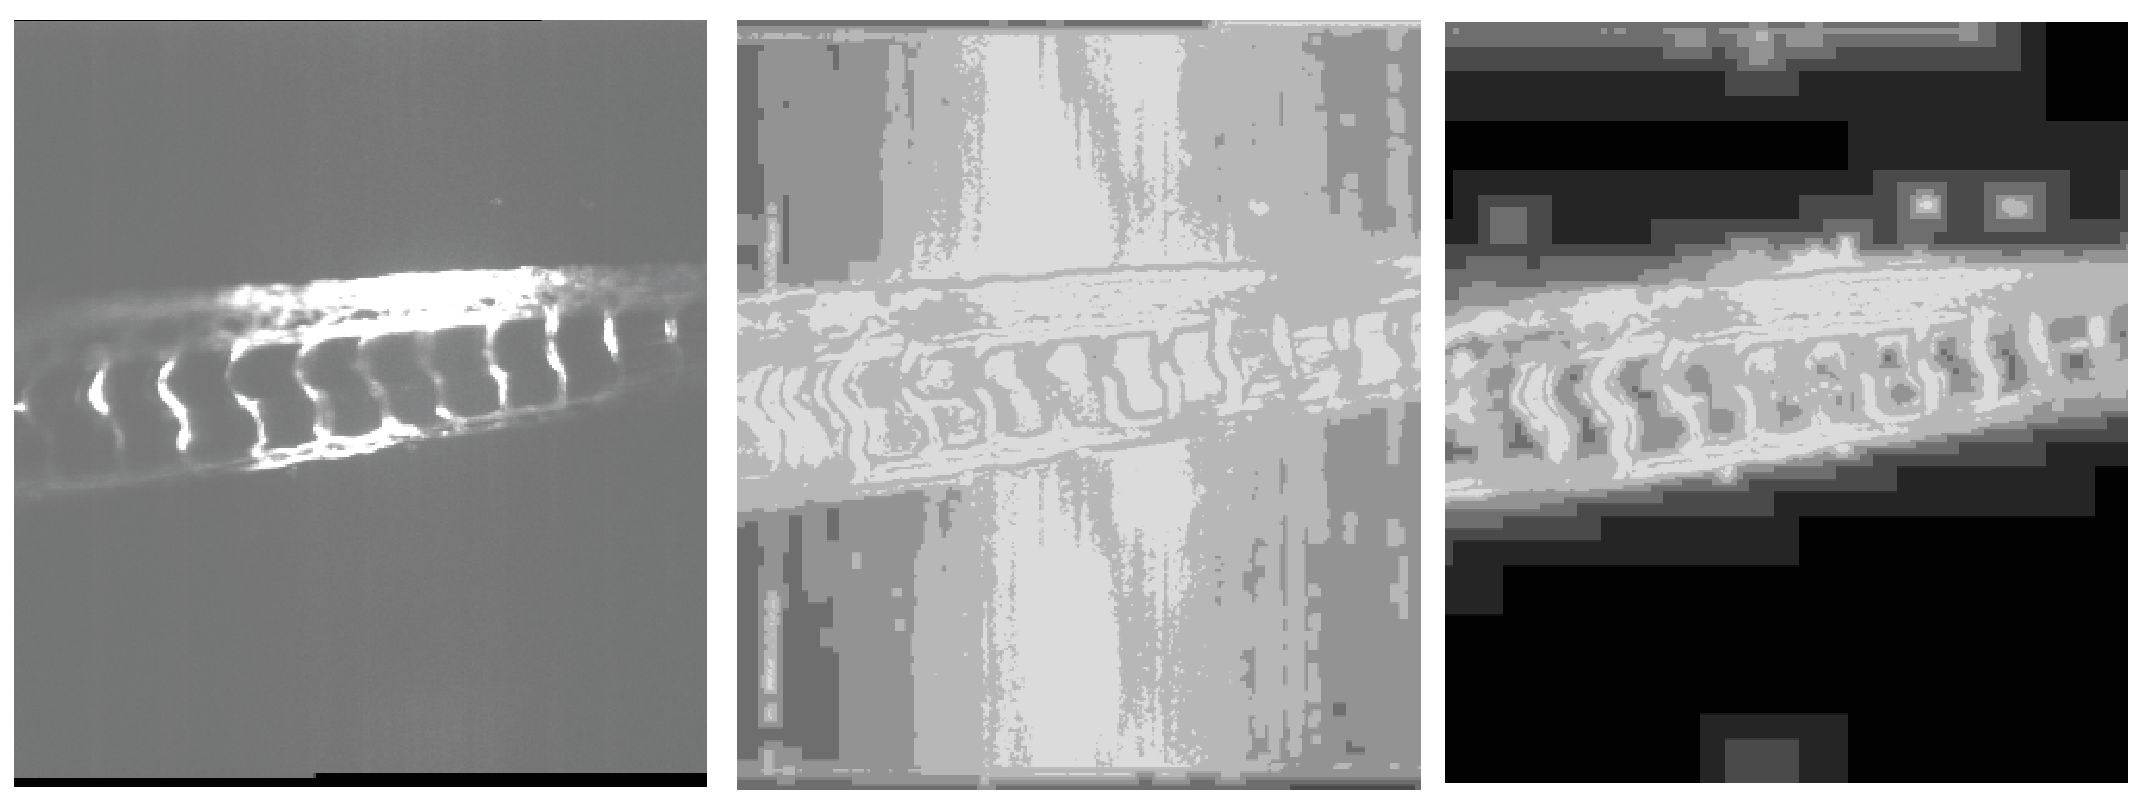
\includegraphics[width=1\textwidth]{level_parameters.pdf}
		\caption{\textbf{Particle Cell Level (local resolution) to visualize APR spatial adaptation and automatic parameters}. Here we show (left) a subsection of input image, (middle) the Particle Cell Level using automatic parameters (-I\_th=952 and -min\_signal=62.3) and Particle Cell level of same region with custom set parameters (-I\_th=1030 and -min\_signal=200) to remove resolution of unwanted background signal. The setting of the parameters results in a three fold reduction in the APR size above the automatic parameters. Image of labelled vasculature of a developing Zebrafish, courtesy of Stephan Daetwyler, Huisken Lab, MPI-CBG and Morgridge Institute for Research, Madison}\label{fig:Figure1}
	\end{center}
\end{figure}

When run without parameters, both the intensity and minimum signal thresholds are estimated from the image statistics assuming a dark noisy background of atleast 5\% of the image and a minimum signal to noise ratio of 6. This is done by estimating the median background intensity noise level, and calculating the standard deviations in local patches. See APRConverter::autoparamters.

This means of setting the paramters is violated if the image does not contain a noisy background, either due to the image modality or pre-processing. The pipeline will attempt to detect situations where the background has a fixed intensity, and will set the parameters to set defaults, assuming the image has no background and a high signal to noise ratio.

Evaluating the adaptaion of the APR for a given dataset can be done through observing the Particle Cell level, which is output as a down-sampled tif image when using Example\_get\_apr. The Particle Cell level represents the local resolution the image is resolved at, with a change of level representing a halfing of resolution in each direction. The adaptation can be in more detailed explored by direct reconstruction using Example\_reconstruct\_image

Although we have found that the automatic parameters provide good estimates across a wide variety of examples, getting the greatest accuracy, and memory and computational reductions requires tailoring the image parameters. In paticular, the image intensity and minimum signal can be adjusted to remove un-wanted background or non-relevant signal. In Figure~1, we provide an example, where automatic parameters, result in the inclusion of un-wanted background signal, and setting of custom parameters through viewing the dataset in Fiji result in the APR ignoring the un-wanted signal. The intensity threshold can be easily set by visual inspection of the image through software such as Fiji, setting the value to the highest value such that all required information is above the threshold. Second, the minimum signal can be similarly set, by finding the dimmest object in the image (relative to the local background, not global intensity), that is wished to be resolved. It would be suggested that then the -min\_signal be set to 80\% of the estimated value by eye. Once set, the adaptation can then be again evaluated again by viewing the Particle Cell level and reconstructions as discussed above.
\subsection{Guiding the APR with a mask file}
Lastly, any external information can be used to guide the APR through use of an additional mask image, use the -mask\_file option. This expects an binary image of the same type as the input, where pixels with zero values will be ignored by the adaptation of the APR. The mask file could be generated extenrally, such as in Fiji, or generated within the library.
\section{Processing with the APR}
The APR once created, is stored in memory, using the APR class, see /src/data\_structures/APR/APR.hpp.
\subsection{APR Data-structure}
The APR class consists of two components, the spatial and resolution information of the APR, handled by the APRAccess class, and the particle intensities, stored using the ExtraParticleData class.
\subsubsection{Access Data}
The APRAccess class, stores the Particle Cell spatial co-ordinates, level and type. The spatial co-ordinates and type are stored using a by row, sparse black-red tree, described in more detail in the supplementary material of the APR paper. This structure allows sparse storage of the information while allowing both linear iteration, and random access.
\subsubsection{ExtraParticleData Class}
The ExtraParticleData class, is used for storing particle properties, and simply stores these properties in a contiguous array in memory. The particle intensities are stored in a public data member of the APR called particle\_intensities. Additional particle properties can easily be created, computed, over and stored using this class (See Example\_apr\_iterate).
\subsection{Input-Output}
The APR is stored using hdf5 with BLOSC library (github.com/Blosc/hdf5-blosc) used for compression. Currently, files produced in this way can only be read by the library, as the spatial information is encoded in the form used by the APR datastructures. Alternatively, the APR can be written explicitly, as shown by Example\_produce\_paraview\_file. This file can then be directly read using the produced xmf file in paraview, and in Matlab using the reading script found in matlab\_helpers. Note, that this explicit form requires a larger amount of memory then the standard apr storage.

The speed, and lossless compression rate can be direclty altered by the user when writing APR files.
\subsubsection{Compression}
The particle intensities can be additionally compressed in a lossy manner, as shown in Example\_compress\_apr.
\subsubsection{ExtraParticleData}
Additional particle information is stored seperately in additional hdf5 files, for details see the APRWriter class. 
\section{Data Access and Processing}
The APR is an multi-resolution adaptive representation, and therefore requires additional steps, compared to a pixel image, when iterating over particle information with knowledge of spatial and resolution information. This is handled by the APRIterator class. Note, that this is not a STL type iterator. The iterator, once set, points to a particular particle and Particle Cell, allowing access to full spatial information, type, and access to any particle properties. We outline briefly examples of the iteration below. For more details, and advanced examples, see Example\_apr\_iterate.
\subsection{Serial Iteration}
\begin{lstlisting}
APRIterator<uint16_t> apr_iterator(apr); // not STL type iteration

uint64_t particle_number;
//Basic serial iteration over all particles
for (particle_number = 0; particle_number < apr.total_number_particles(); ++particle_number) {
	//This step is required for all loops to set the iterator by the particle number
	apr_iterator.set_iterator_to_particle_by_number(particle_number);

	//once set you can access all informaiton on the particle cell
	uint64_t current_particle_cell_spatial_index_x = apr_iterator.x();
	uint64_t current_particle_cell_spatial_index_y = apr_iterator.y();
	uint64_t current_particle_cell_spatial_index_z = apr_iterator.z();
	uint64_t current_particle_cell_level = apr_iterator.level();
	uint64_t current_particle_cell_type = apr_iterator.type();
	
	//you can also query the global co-ordinate of the particle (or center of Particle Cell)
	float particle_global_coordinate_x = apr_iterator.x_global();
	
	//This is how ExtraParticleData is accessed, in paticular this is how the particle intensities are accessed.
	uint16_t current_particle_intensity = apr.particle_intensities[apr_iterator];

}
\end{lstlisting}
Other modes of iteration, by level, and z or x, can also be done and are shown by example in Example\_apr\_iterate.
\subsection{Parallel Iteration}
The only difference with parallel iteration, is the inclusion of the OpenMP pragma which requires that the particle number be private, and the iterator be firstprivate. This can be simple done as follows:
\begin{lstlisting}
APRIterator<uint16_t> apr_iterator(apr); // not STL type iteration

ExtraParticleData<uint8_t> threshold_particles(apr); // We create another particle property to store a particle threshold

uint16_t threshold = 100;

//Note making the particle_number private, and apr_iterator first private are required, and static schedule suggested.
#pragma omp parallel for schedule(static) private(particle_number) firstprivate(apr_iterator)
for (particle_number = 0; particle_number < apr_iterator.total_number_particles(); ++particle_number) {
	//needed step for any loop (update to the next part)
	apr_iterator.set_iterator_to_particle_by_number(particle_number);

	//All particle properties are accessed as in the serial example above,
	if(apr.particle_intensities[apr_iterator] > threshold){
		threshold_particles[apr_iterator] = 1; // If the intensity is greater then the threshold set the threshold particle property to 1.
	} else {
		threshold_particles[apr_iterator] = 0; // Otherwise set the particle property to 0.
	}
}
\end{lstlisting}
\subsection{Neighbor Iteration}
The second form of important iteration, is that of particle neighbours. The library currently provides support for only accessing the direct face neighbours of a Particle Cell. This means there are 6 directions, and in each direction we know that the Particle Cell can either be on the same level, a level lower (lower resolution), or a level higher (higher resolution). In the case of the same or lower, there is only one neighbour, in the case of higher resolution there are four neighbors in each direction.

Neighbor access is handled by the use of an additional APRIterator, which we call the neighbour iterator. This can then be used to access particle properties in same way as usual iteration, and also to access particle properties stored in ExtraParticleData. Below we give an example of summing the neighbours intensities, and multiplying that by the difference of the y values of the particle location.
\begin{lstlisting}
ExtraParticleData<float> neighbor_sum(apr); // Additional float Particle Property for storing the sum of the neighbours

APRIterator<uint16_t> neighbour_iterator(apr);
APRIterator<uint16_t> apr_iterator(apr);

//Basic serial iteration over all particles
uint64_t particle_number;

#pragma omp parallel for schedule(static) private(particle_number) firstprivate(apr_iterator,neighbour_iterator)
for (particle_number = 0; particle_number < apr_iterator.total_number_particles(); ++particle_number) {
	//needed step for any loop (update to the next part)
	apr_iterator.set_iterator_to_particle_by_number(particle_number);

	//loop over all the neighbours and set the neighbour iterator to it
	for (int direction = 0; direction < 6; ++direction) {
		apr_iterator.find_neighbours_in_direction(direction);
		// Neighbour Particle Cell Face definitions [+y,-y,+x,-x,+z,-z] =  [0,1,2,3,4,5]
		for (int index = 0; index < apr_iterator.number_neighbours_in_direction(direction); ++index) {

			if(neighbour_iterator.set_neighbour_iterator(apr_iterator, direction, index)){
				//neighbour_iterator works just like apr, and apr_iterator (you could also call neighbours)
				neighbor_sum[apr_iterator] += apr.particles_intensities[neighbour_iterator]*(apr_iterator.y_global() - neighbour_iterator.y_global());
			}
		}
	}
}
\end{lstlisting}
\subsection{Random access}
In the above examples, we have shown methods for iterating through the particles in a specified order. The datastructure also allows, almost $\mathcal{O}(1)$ data access (The exact relationship is content and size dependent, please see the supplimentary material of the main paper). Example\_random\_access provides examples on its use.
\subsection{Particle Transforms}
In addition to being able to iterate over each particle with full information, if only a simple operation is requried directly on one, or two particle properties, optimized routines can be used that utilize C++ std::transform functionality. These are the map, map\_inplace, zip, and zip\_inplace functions, and we direct the user to Example\_apr\_iterate for examples. These functions allow for the computation of simple operations in a very efficient, and parallel manner, with only a single line of code. For example, here we simply take the absolute value of a the particle intensities and store it as a new particle property:
\begin{lstlisting}
ExtraParticleData<uint16_t> absolute_value_of_intensities;
//return the absolute value of the part dataset (includes initialization of the output result)
apr.particle_intensities.map(apr,absolute_value_of_intensities,[](const uint16_t &a) { return abs(a); });
\end{lstlisting}
\section{Pixel Images and Reconstruction}
Pixel images are handled using the MeshData class and tiff library is used for input-output.
\subsection{Reconstruction}
Any particle property, stored using ExtraParticleData class, can be interpolated to reconstruct an image, allowing both a piecewise constant and smooth reconstruction. For examples see Example\_reconstruct\_image.
\subsection{Sampling particles from an image}
In addition, particle properties can be sampled from an input image, using the get\_parts\_from\_img, member function of the APR class.
\section{Processing Examples}
We provide some simple examples of processing on the APR in Example\_ray\_cast and Example\_compute\_gradient.
\section{Visualization}
The APR can be visualized using the Example\_ray\_cast, and using Paraview using the Example\_produce\_paraview\_file.
\section{Coming Soon}
The library is still in active development, and additional features, algorithm, and support, will be continuously added going forward. If there are any features you would like included, please get in touch with us, either by email or through the github repository.

Features that are in the works include:
\begin{itemize}
	\item APR Segmentation
	\item APR Tree structure
	\item APR Pixel based filtering
	\item Fiji Support, including integration of visualization using Scenery.
\end{itemize}
\end{document}
